\documentclass[11pt]{article}
\usepackage{amsmath,amssymb}
\usepackage{graphics}
\usepackage{graphicx}
\newcommand{\numpy}{{\tt numpy}}    % tt font for numpy

\topmargin -.5in
\textheight 9in
\oddsidemargin -.25in
\evensidemargin -.25in
\textwidth 7in

\begin{document}

% ========== Edit your name here
\author{Daniel López - Heber Orellana - Anderson Peña} \date{\today}
\title{Map 1: Curvas de Bezier}
\maketitle

\medskip

% ========== Begin answering questions here
\begin{enumerate}

\item
Curva de bezier de los puntos de control: $P_0(4,1)$, $P_1(28,48)$, $P_3(50,42)$, $P_4(40,5)$
% ========== Just examples, please delete before submitting 
Grafica:
%\begin{figure}
%%==\includegraphics[scale=25]{grafica1.png}
%\caption{Curva de bezier y puntos}
%\label{fig: grafica1}
%\end{figure}

\item
Grafica con segmento de recta $\overline{P_0 P_1}$, $\overline{P_1 P_2}$, $\overline{P_2 P_3}$
% ========== Continue adding items as needed

\begin{center}
	\begin{figure}[h!]
		\centering
		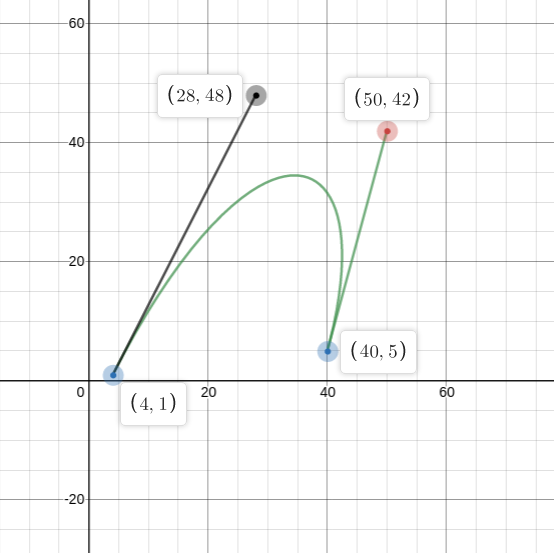
\includegraphics[width=50mm]{Ejercicio1.png}
		\caption{Grafica cubriendo preguntas 1 y 2}
	\end{figure}
\end{center}

\item
Demostracion de tangente en $P_0$ pasa por $P_1$ y la recta tangente de  $P_3$ pasa por $P_2$


\item 
Demostración con letra \emph{C}
\begin{center}
	\begin{figure}[h!]
		\centering
		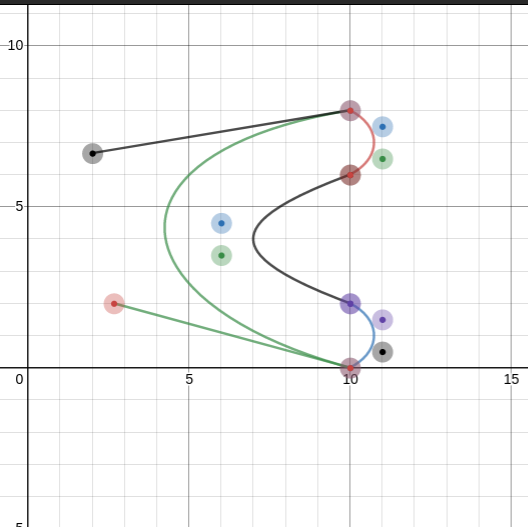
\includegraphics[width=50mm]{LetraCC.png}
	\end{figure}
\end{center}
Ecuaciones que conforman la letra \emph{C}
\begin{equation}
f(x) = 8(1-t)^3 + 20t(1-t)^2 + 6t^2(1-t)+ 0t^3 
\end{equation}
\begin{equation}
f(y) = 10(1-t)^3 + 6t(1-t)^2 + 8t^2(1-t)+ 10t^3 
\end{equation}
\begin{equation}
f(x) = 11(1-t)^3 + 33t(1-t)^2 +33t^2(1-t)+ 10t^3 
\end{equation}
\begin{equation}
f(y) = 9(1-t)^3 + 22.5t(1-t)^2 + 19.5t^2(1-t)+ 6t^3 
\end{equation}
\begin{equation}
f(x) = 10(1-t)^3 + 12t(1-t)^2 + 12t^2(1-t)+ 10t^3 
\end{equation}
\begin{equation}
f(y) = 6(1-t)^3 + 13.5t(1-t)^2 + 10.5t^2(1-t)+ 2t^3 
\end{equation}
\begin{equation}
f(x) = 10(1-t)^3 + 33t(1-t)^2 + 33t^2(1-t)+ 10t^3 
\end{equation}
\begin{equation}
f(y) = 2(1-t)^3 + 4.5t(1-t)^2 + 1.5t^2(1-t)+ 0t^3 
\end{equation}

\item 
Apellido del matemático: \emph{Carter}
Letra \emph{C}
\begin{equation}
f(x) = 8(1-t)^3 + 20t(1-t)^2 + 6t^2(1-t)+ 0t^3 
\end{equation}
\begin{equation}
f(y) = 10(1-t)^3 + 6t(1-t)^2 + 8t^2(1-t)+ 10t^3 
\end{equation}
\begin{equation}
f(x) = 11(1-t)^3 + 33t(1-t)^2 +33t^2(1-t)+ 10t^3 
\end{equation}
\begin{equation}
f(y) = 9(1-t)^3 + 22.5t(1-t)^2 + 19.5t^2(1-t)+ 6t^3 
\end{equation}
\begin{equation}
f(x) = 10(1-t)^3 + 12t(1-t)^2 + 12t^2(1-t)+ 10t^3 
\end{equation}
\begin{equation}
f(y) = 6(1-t)^3 + 13.5t(1-t)^2 + 10.5t^2(1-t)+ 2t^3 
\end{equation}
\begin{equation}
f(x) = 10(1-t)^3 + 33t(1-t)^2 + 33t^2(1-t)+ 10t^3 
\end{equation}
\begin{equation}
f(y) = 2(1-t)^3 + 4.5t(1-t)^2 + 1.5t^2(1-t)+ 0t^3 
\end{equation}
Letra \emph{A}
\begin{equation}
f(x)= (1-t)^{3}\left(12\right)+3t(1-t)^{2}\left(12\right)+3t^{2}(1-t)\left(18\right)+t^{3}\left(18\right)
\end{equation}
\begin{equation}
f(y)=(1-t)^{3}\left(0\right)+3t(1-t)^{2}\left(10\right)+3t^{2}(1-t)\left(10\right)+t^{3}\left(0\right)
\end{equation}
\begin{equation}
f(x)=(1-t)^{3}\left(13\right)+3t(1-t)^{2}\left(13\right)+3t^{2}(1-t)\left(17\right)+t^{3}\left(17\right)
\end{equation}
\begin{equation}
f(y)=(1-t)^{3}\left(0\right)+3t(1-t)^{2}\left(8\right)+3t^{2}(1-t)\left(8\right)+t^{3}\left(0\right)
\end{equation}
\begin{equation}
f(x)=(1-t)^{3}\left(12\right)+3t(1-t)^{2}\left(14\right)+3t^{2}(1-t)\left(16\right)+t^{3}\left(18\right)
\end{equation}
\begin{equation}
f(y)=(1-t)^{3}\left(3.5\right)+3t(1-t)^{2}\left(4\right)+3t^{2}(1-t)\left(4\right)+t^{3}\left(3.5\right)
\end{equation}

\begin{equation}
f(x)=(1-t)^{3}\left(12\right)+3t(1-t)^{2}\left(14\right)+3t^{2}(1-t)\left(16\right)+t^{3}\left(18\right)
\end{equation}
\begin{equation}
f(y)=(1-t)^{3}\left(3.5\right)+3t(1-t)^{2}\left(3\right)+3t^{2}(1-t)\left(3\right)+t^{3}\left(3.5\right)
\end{equation}
Letra \emph{R}
\begin{equation}
	f(x) = (1-t)^{3}\left(19\right)+3t(1-t)^{2}\left(19\right)+3t^{2}(1-t)\left(19\right)+t^{3}\left(19\right)
\end{equation}

\begin{equation}
f(y) = (1-t)^{3}\left(0\right)+3t(1-t)^{2}\left(3\right)+3t^{2}(1-t)\left(3\right)+t^{3}\left(7.5\right)
\end{equation}

\begin{equation}
f(x) = (1-t)^{3}\left(19\right)+3t(1-t)^{2}\left(24\right)+3t^{2}(1-t)\left(24\right)+t^{3}\left(20\right) 
\end{equation}
\begin{equation}
f(y) = (1-t)^{3}\left(7.5\right)+3t(1-t)^{2}\left(7.5\right)+3t^{2}(1-t)\left(3\right)+t^{3}\left(3\right)
\end{equation}

\begin{equation}
f(x) = (1-t)^{3}\left(20\right)+3t(1-t)^{2}\left(22\right)+3t^{2}(1-t)\left(22\right)+t^{3}\left(20\right)
\end{equation}

\begin{equation}
f(y) = (1-t)^{3}\left(6.5\right)+3t(1-t)^{2}\left(6.5\right)+3t^{2}(1-t)\left(4\right)+t^{3}\left(4\right)
\end{equation}

\begin{equation}
f(x) = (1-t)^{3}\left(20\right)+3t(1-t)^{2}\left(20\right)+3t^{2}(1-t)\left(20\right)+t^{3}\left(20\right)
\end{equation}

\begin{equation}
f(y) = (1-t)^{3}\left(6.5\right)+3t(1-t)^{2}\left(6\right)+3t^{2}(1-t)\left(5\right)+t^{3}\left(4\right)
\end{equation}

\begin{equation}
f(x)=(1-t)^{3}\left(20\right)+3t(1-t)^{2}\left(20\right)+3t^{2}(1-t)\left(20\right)+t^{3}\left(20\right)
\end{equation}

\begin{equation}
f(y)=(1-t)^{3}\left(6.5\right)+3t(1-t)^{2}\left(6\right)+3t^{2}(1-t)\left(5\right)+t^{3}\left(4\right)
\end{equation}

\begin{equation}
f(x) = (1-t)^{3}\left(20\right)+3t(1-t)^{2}\left(20\right)+3t^{2}(1-t)\left(20\right)+t^{3}\left(20\right)
\end{equation}

\begin{equation}
f(y) = (1-t)^{3}\left(0\right)+3t(1-t)^{2}\left(2\right)+3t^{2}(1-t)\left(2\right)+t^{3}\left(2\right)
\end{equation}

\begin{equation}
f(x) = (1-t)^{3}\left(20\right)+3t(1-t)^{2}\left(21\right)+3t^{2}(1-t)\left(22\right)+t^{3}\left(22.5\right)
\end{equation}

\begin{equation}
f(y) = (1-t)^{3}\left(3\right)+3t(1-t)^{2}\left(2\right)+3t^{2}(1-t)\left(1\right)+t^{3}\left(0\right)
\end{equation}

\begin{equation}
f(x) = (1-t)^{3}\left(20\right)+3t(1-t)^{2}\left(21\right)+3t^{2}(1-t)\left(21.5\right)+t^{3}\left(21.7\right)
\end{equation}

\begin{equation}
f(y) = (1-t)^{3}\left(2\right)+3t(1-t)^{2}\left(1\right)+3t^{2}(1-t)\left(0.5\right)+t^{3}\left(0\right)
\end{equation}

Letra \emph{T}

\begin{equation}
f(x) = (1-t)^{3}\left(24\right)+3t(1-t)^{2}\left(26\right)+3t^{2}(1-t)\left(27\right)+t^{3}\left(28\right)
\end{equation}
\begin{equation}
f(y) = (1-t)^{3}\left(6\right)+3t(1-t)^{2}\left(6\right)+3t^{2}(1-t)\left(6\right)+t^{3}\left(6\right)
\end{equation}

\begin{equation}
f(x) = (1-t)^{3}\left(24\right)+3t(1-t)^{2}\left(26\right)+3t^{2}(1-t)\left(27\right)+t^{3}\left(28\right)
\end{equation}

\begin{equation}
f(y) = (1-t)^{3}\left(6\right)+3t(1-t)^{2}\left(6\right)+3t^{2}(1-t)\left(6\right)+t^{3}\left(6\right)
\end{equation}

\begin{equation}
f(x) = (1-t)^{3}\left(24\right)+3t(1-t)^{2}\left(26\right)+3t^{2}(1-t)\left(27\right)+t^{3}\left(28\right)
\end{equation}
\begin{equation}
f(y) = (1-t)^{3}\left(5\right)+3t(1-t)^{2}\left(5\right)+3t^{2}(1-t)\left(5\right)+t^{3}\left(5\right)
\end{equation}
\begin{equation}
f(x) = (1-t)^{3}\left(24\right)+3t(1-t)^{2}\left(23.5\right)+3t^{2}(1-t)\left(23.5\right)+t^{3}\left(24\right)
\end{equation}

\begin{equation}
f(y) = (1-t)^{3}\left(6\right)+3t(1-t)^{2}\left(5.75\right)+3t^{2}(1-t)\left(5.25\right)+t^{3}\left(5\right)
\end{equation}
\begin{equation}
f(x) = (1-t)^{3}\left(28\right)+3t(1-t)^{2}\left(28.5\right)+3t^{2}(1-t)\left(28.5\right)+t^{3}\left(28\right)
\end{equation}
\begin{equation}
f(y) = (1-t)^{3}\left(6\right)+3t(1-t)^{2}\left(5.75\right)+3t^{2}(1-t)\left(5.25\right)+t^{3}\left(5\right)
\end{equation}
\begin{equation}
f(x) = (1-t)^{3}\left(25\right)+3t(1-t)^{2}\left(25\right)+3t^{2}(1-t)\left(25\right)+t^{3}\left(25\right)
\end{equation}
\begin{equation}
f(y) = (1-t)^{3}\left(0\right)+3t(1-t)^{2}\left(4\right)+3t^{2}(1-t)\left(6\right)+t^{3}\left(7\right)
\end{equation}

\begin{equation}
f(x) = (1-t)^{3}\left(27\right)+3t(1-t)^{2}\left(27\right)+3t^{2}(1-t)\left(27\right)+t^{3}\left(27\right)
\end{equation}
\begin{equation}
f(y) = (1-t)^{3}\left(0\right)+3t(1-t)^{2}\left(4\right)+3t^{2}(1-t)\left(6\right)+t^{3}\left(7\right)
\end{equation}
\begin{equation}
f(x) = (1-t)^{3}\left(25\right)+3t(1-t)^{2}\left(25.5\right)+3t^{2}(1-t)\left(26.5\right)+t^{3}\left(27\right)
\end{equation}
\begin{equation}
f(y) = (1-t)^{3}\left(7\right)+3t(1-t)^{2}\left(7.5\right)+3t^{2}(1-t)\left(7.5\right)+t^{3}\left(7\right)
\end{equation}
\begin{equation}
f(x) = (1-t)^{3}\left(29\right)+3t(1-t)^{2}\left(29\right)+3t^{2}(1-t)\left(35\right)+t^{3}\left(35\right)
\end{equation}
\begin{equation}
f(y) = (1-t)^{3}\left(0\right)+3t(1-t)^{2}\left(10\right)+3t^{2}(1-t)\left(10\right)+t^{3}\left(0\right)
\end{equation}
Letra \emph{A}
\begin{equation}
f(x) = (1-t)^{3}\left(29\right)+3t(1-t)^{2}\left(29\right)+3t^{2}(1-t)\left(35\right)+t^{3}\left(35\right)
\end{equation}
\begin{equation}
f(y) = (1-t)^{3}\left(0\right)+3t(1-t)^{2}\left(10\right)+3t^{2}(1-t)\left(10\right)+t^{3}\left(0\right)
\end{equation}
\begin{equation}
f(x) = (1-t)^{3}\left(30\right)+3t(1-t)^{2}\left(30\right)+3t^{2}(1-t)\left(34\right)+t^{3}\left(34\right)
\end{equation}
\begin{equation}
f(y) = (1-t)^{3}\left(0\right)+3t(1-t)^{2}\left(8\right)+3t^{2}(1-t)\left(8\right)+t^{3}\left(0\right)
\end{equation}
\begin{equation}
f(x) = (1-t)^{3}\left(29\right)+3t(1-t)^{2}\left(31\right)+3t^{2}(1-t)\left(33\right)+t^{3}\left(35\right)
\end{equation}
\begin{equation}
f(y) = (1-t)^{3}\left(3.5\right)+3t(1-t)^{2}\left(4\right)+3t^{2}(1-t)\left(4\right)+t^{3}\left(3.5\right)
\end{equation}
\begin{equation}
f(x) = (1-t)^{3}\left(29\right)+3t(1-t)^{2}\left(31\right)+3t^{2}(1-t)\left(33\right)+t^{3}\left(35\right)
\end{equation}
\begin{equation}
f(y) = (1-t)^{3}\left(3.5\right)+3t(1-t)^{2}\left(4\right)+3t^{2}(1-t)\left(4\right)+t^{3}\left(3.5\right)
\end{equation}

\begin{equation}
f(x) = (1-t)^{3}\left(29\right)+3t(1-t)^{2}\left(31\right)+3t^{2}(1-t)\left(33\right)+t^{3}\left(35\right)
\end{equation}
\begin{equation}
f(y) = (1-t)^{3}\left(3.5\right)+3t(1-t)^{2}\left(3\right)+3t^{2}(1-t)\left(3\right)+t^{3}\left(3.5\right)
\end{equation}

Letra \emph{N}
\begin{equation}
f(x) = (1-t)^{3}\left(36\right)+3t(1-t)^{2}\left(39\right)+3t^{2}(1-t)\left(42\right)+t^{3}\left(44\right)
\end{equation}
\begin{equation}
f(y) = (1-t)^{3}\left(0\right)+3t(1-t)^{2}\left(8\right)+3t^{2}(1-t)\left(8\right)+t^{3}\left(0\right)
\end{equation}
\begin{equation}
f(x) = (1-t)^{3}\left(38\right)+3t(1-t)^{2}\left(39\right)+3t^{2}(1-t)\left(41\right)+t^{3}\left(42\right)
\end{equation}
\begin{equation}
f(y) = (1-t)^{3}\left(0\right)+3t(1-t)^{2}\left(5\right)+3t^{2}(1-t)\left(5\right)+t^{3}\left(0\right)
\end{equation}

\begin{equation}
f(x) = (1-t)^{3}\left(36\right)+3t(1-t)^{2}\left(36\right)+3t^{2}(1-t)\left(36\right)+t^{3}\left(36\right)
\end{equation}
\begin{equation}
f(y) = (1-t)^{3}\left(0\right)+3t(1-t)^{2}\left(3\right)+3t^{2}(1-t)\left(3\right)+t^{3}\left(6\right)
\end{equation}
\begin{equation}
f(x) = (1-t)^{3}\left(37\right)+3t(1-t)^{2}\left(37\right)+3t^{2}(1-t)\left(37\right)+t^{3}\left(37\right)
\end{equation}
\begin{equation}
f(y) = (1-t)^{3}\left(2.4\right)+3t(1-t)^{2}\left(3\right)+3t^{2}(1-t)\left(3\right)+t^{3}\left(6\right)
\end{equation}
\begin{equation}
f(x) = (1-t)^{3}\left(36\right)+3t(1-t)^{2}\left(36.25\right)+3t^{2}(1-t)\left(36.75\right)+t^{3}\left(37\right)
\end{equation}
\begin{equation}
f(y) = (1-t)^{3}\left(6\right)+3t(1-t)^{2}\left(6.25\right)+3t^{2}(1-t)\left(6.25\right)+t^{3}\left(6\right)
\end{equation}

\begin{center}
	\begin{figure}[h!]
		\centering
		\includegraphics[width=200mm]{Cartan.png}
		\caption{Nombre de Henri Cartan}
	\end{figure}
\end{center}

\end{enumerate}

\end{document}
\grid
\grid